\documentclass[12pt]{article}
%Gumm{\color{blue}i}|065|=)
\usepackage{amsmath, amsfonts, amssymb}
\usepackage[margin=0.5in]{geometry}
\usepackage{xcolor}
\usepackage{graphicx}
\usepackage{amsmath}

\newcommand{\off}[1]{}
\DeclareMathSizes{20}{30}{20}{18}
\usepackage{tikz}


\title{Scratchwork: Class Field Theory}
\date{}
\begin{document}

\sffamily

\maketitle

\noindent One common mistake is to say the ring of integers of $K =  \mathbb{Q}(\sqrt{-5})$ is $\mathbb{Z}[\sqrt{-5}]$.  In fact it's $\mathbb{Z}[\frac{1+\sqrt{-5}}{2}]$. This example is important because it's the first time we observe the failure of unique factorization in ``integers":
$$2 \times 3 = (1 + \sqrt{-5}) \times (1 - \sqrt{-5}) $$
Despite being quite well-known, I feel this is the kind of result that needs to be checked very carefully.  Number Theory in particular, is known to re-arrange obvious facts in shocking ways:
$$ \left( \frac{1 + \sqrt{-5}}{2} \right)^2 = \frac{1}{4} + \sqrt{-5} - \frac{5}{4} 
= 2 \times \left( \frac{1 + \sqrt{-5}}{2} \right) - 2 \times 1$$
What's so special about the $\sqrt{-5}$ that we obtain a number field with class number $h(K)=2$ ? \\ \\
\textbf{Ex} Factor the numbers $1 \leq n \leq 100$ in each of the two orders, $\mathcal{O}_1 = \mathbb{Z}\left[ \frac{1 + \sqrt{-5}}{2}\right]$ and $\mathcal{O}_2 = \mathbb{Z}[\sqrt{-5}]$. \\ \\
\textbf{Ex} Show that the ring of integers of $\mathbb{Q}(\sqrt{-5})$ is $\mathbb{Z}\left[ \frac{1 + \sqrt{-5}}{2}\right]$. \\ \\
Let's try to draw the ideal $(2)$. \\ \\
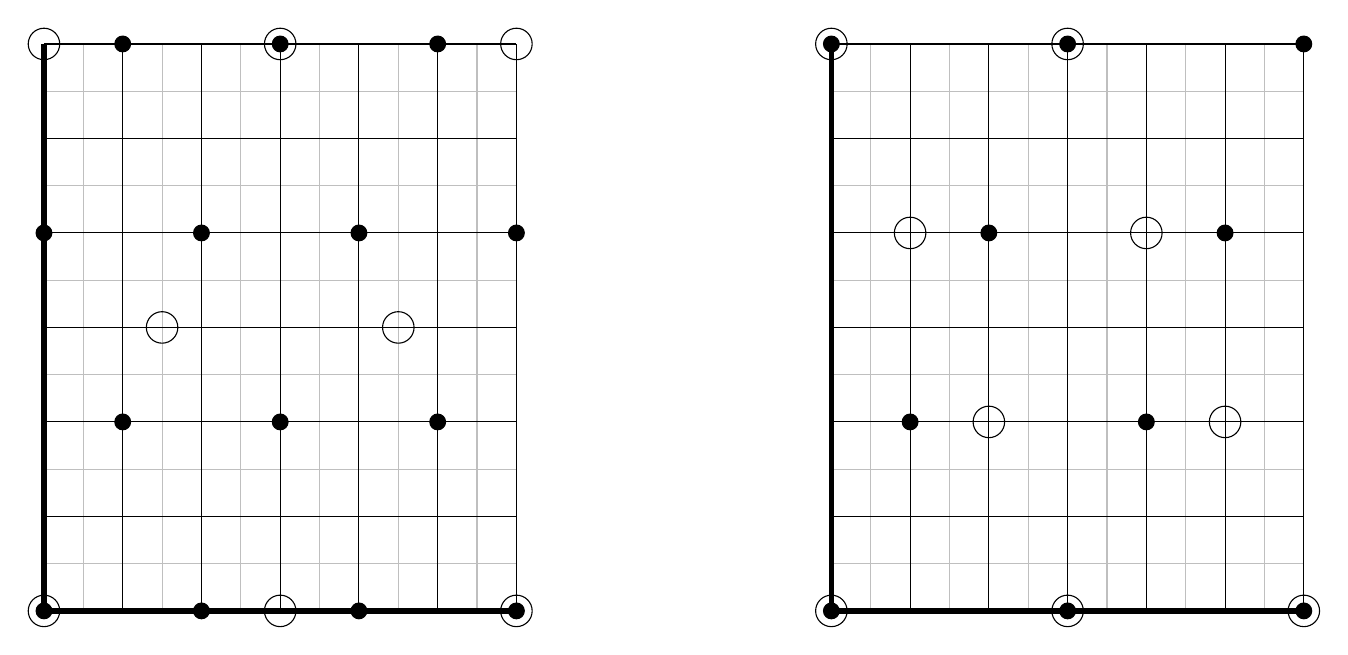
\begin{tikzpicture}[scale=1]

\begin{scope}


\foreach \a in {0,0.5,...,6}{
	\draw[black!25!white] (\a, 0)--(\a,6*1.2);
}

\foreach \a in {0,0.5,...,6}{
	\draw[black!25!white] (0,\a*1.2)--(6,\a*1.2);
}

\foreach \a in {0,...,6}{
	\draw (\a, 0)--(\a,6*1.2);
}

\foreach \a in {0,...,6}{
	\draw (0,\a*1.2)--(6,\a*1.2);
}

\draw[line width=2] (0,0)--(0,6*1.2);
\draw[line width=2] (0,0)--(6,0);

\draw[fill=black] (0,0*1.2) circle (0.1);
\draw[fill=black] (2,0*1.2) circle (0.1);
\draw[fill=black] (4,0*1.2) circle (0.1);
\draw[fill=black] (6,0*1.2) circle (0.1);

\draw[fill=black] (1,2*1.2) circle (0.1);
\draw[fill=black] (3,2*1.2) circle (0.1);
\draw[fill=black] (5,2*1.2) circle (0.1);

\draw[fill=black] (0,4*1.2) circle (0.1);
\draw[fill=black] (2,4*1.2) circle (0.1);
\draw[fill=black] (4,4*1.2) circle (0.1);
\draw[fill=black] (6,4*1.2) circle (0.1);

\draw[fill=black] (1,6*1.2) circle (0.1);
\draw[fill=black] (3,6*1.2) circle (0.1);
\draw[fill=black] (5,6*1.2) circle (0.1);

\draw (0,0*1.2) circle (0.2);
\draw (3,0*1.2) circle (0.2);
\draw (6,0*1.2) circle (0.2);

\draw (1.5, 3*1.2) circle (0.2);
\draw (4.5, 3*1.2) circle (0.2);

\draw (0,6*1.2) circle (0.2);
\draw (3,6*1.2) circle (0.2);
\draw (6,6*1.2) circle (0.2);

\end{scope}

\begin{scope}[xshift=10cm]


\foreach \a in {0,0.5,...,6}{
	\draw[black!25!white] (\a, 0)--(\a,6*1.2);
}

\foreach \a in {0,0.5,...,6}{
	\draw[black!25!white] (0,\a*1.2)--(6,\a*1.2);
}

\foreach \a in {0,...,6}{
	\draw (\a, 0)--(\a,6*1.2);
}

\foreach \a in {0,...,6}{
	\draw (0,\a*1.2)--(6,\a*1.2);
}

\draw[line width=2] (0,0)--(0,6*1.2);
\draw[line width=2] (0,0)--(6,0);

\draw[fill=black] (0,0*1.2) circle (0.1);
\draw[fill=black] (1,2*1.2) circle (0.1);
\draw[fill=black] (2,4*1.2) circle (0.1);
\draw[fill=black] (3,6*1.2) circle (0.1);

%\draw[fill=black] (-2,2*1.2) circle (0.1);
%\draw[fill=black] (-1,4*1.2) circle (0.1);
\draw[fill=black] ( 0,6*1.2) circle (0.1);

\draw[fill=black] (3,0*1.2) circle (0.1);
\draw[fill=black] (4,2*1.2) circle (0.1);
\draw[fill=black] (5,4*1.2) circle (0.1);
\draw[fill=black] (6,6*1.2) circle (0.1);

\draw[fill=black] (6,0*1.2) circle (0.1);

\draw (0,0) circle (0.2);
\draw (3,0) circle (0.2);
\draw (6,0) circle (0.2);

\draw (2,2*1.2) circle (0.2);
\draw (1,4*1.2) circle (0.2);
\draw (0,6*1.2) circle (0.2);

\draw (5,2*1.2) circle (0.2);
\draw (4,4*1.2) circle (0.2);
\draw (3,6*1.2) circle (0.2);



\end{scope}

\end{tikzpicture} \\ \\
Also $(3)$ and on the right hand side $(1 + \sqrt{-5})$ and $(1-\sqrt{-5})$. \\ \\
That was much harder than it should have been.  Btw, do you believe this?  This is what happens when we use a calculator and get the correct answer.  And it's perfectly good.

\begin{verbatim}
>>> 5**0.5/2
1.118033988749895
\end{verbatim}

\newpage

\noindent \textbf{10/06} What is the ring of integers anyway?  \\ \\
\textbf{Def} Let $A \subseteq B$ be an extension of rings. An element $b \in B$ is called \textbf{integral} over $A$ if it satisfies a monic equation:
$$  x^n + a_1 \, x^{n-1} + \dots + a_0 = 0 $$
with coefficients in $a_i \in A$.  The ring $B$ is called \textbf{integral} over $A$ if all its elements $b \in B$ are integral over $A$. \\ \\
Seems like a lot of effort to find new classes of integers.  $(\sqrt{-5})^2 + 5 = 0$ so that $\sqrt{-5}$ is integral over $\mathbb{Z}$.  Any element of $\mathbb{Q}(\sqrt{-5})$ is the root of a quadratic over $\mathbb{Q}$, at least.
$$ (a + b \sqrt{-5})^2 = a^2 + 5b^2 + 2 \sqrt{-5} \, ab = 2a(a + b \sqrt{-5}) + ( - a^2 + 5b^2) $$
Don't you think this algebra is tedious?  So let's have this other definition of integrality: \\ \\
\textbf{Thm} Finintely many elements $b_1, \dots, b_n \in B$ are all integral over $A$ if and only if the ring $A[b_1, \dots, b_n]$ viewed as an $A$-module is finitely generated. \\ \\
Here's another non-constructive argument that you only need a quadratic: $ (a+b\sqrt{-5})^2 \in (a + b \sqrt{-5}) \, \mathbb{Q}\oplus 1 \, \mathbb{Q}$, so there must be a quadratic relation.  Modern algbra is frustratingly succinct but at least we didn't have to solve anything. \\ \\
We can represent elements of $\mathbb{Q}(\sqrt{-5})$ as $2 \times 2$ matrices using a straightforward device:
$$ a + b \sqrt{-5} \mapsto \left[ \begin{array}{cc} a & b \\ 5b & a \end{array} \right] $$
As a $2 \times 2$ matrix we could use the \textbf{Cayley-Hamilton theorem} we have that $I$ and $A$ and $A^2$ must have a relation over $\mathbb{Q}$.  This machinery is a bit over-powerful if we only solve Pell-type equations with it.  In fact, it makes no sense to use adjoint matrices until $3 \times 3$.  
$$ \left[ \begin{array}{ccc} a & b & c \\ d & e & f \\ g & h & i\end{array} \right]
\mapsto \left[ \begin{array}{ccc} 
\left| \begin{array}{cc} e & f \\ h & i\end{array} \right|  & 
\left| \begin{array}{cc} d & f \\ g & i\end{array} \right|  & 
\left| \begin{array}{cc} d & e \\ g & h\end{array} \right|  \\ \\
\left| \begin{array}{cc} a & b \\ h & i\end{array} \right|  & 
\left| \begin{array}{cc} a & c \\ g & i\end{array} \right|  & 
\left| \begin{array}{cc} b & c \\ g & h\end{array} \right|  \\ \\
\left| \begin{array}{cc} a & b \\ e & f\end{array} \right|  & 
\left| \begin{array}{cc} a & c \\ d & f\end{array} \right|  & 
\left| \begin{array}{cc} b & c \\ d & e\end{array} \right|  \end{array} \right] $$
Wikipedia returns this formula for the $2 \times 2$ and $3 \times 3$ adjoint matrix.\footnote{\texttt{https://en.wikipedia.org/wiki/Adjugate\_{}matrix}} and Linear Algebra formula exist in abundance.  We never use them.
$$ A^* = I (\text{tr} A) - A \quad(2 \times 2)\quad\text{or}\quad A^* = \frac{1}{2}\big( (\text{tr}A)^2 - \text{tr}(A^2) \big) - A (\text{tr}A) + A^2\quad(3 \times 3) $$
It seems awfully odd we don't check the cubic case.  We might use a computer, in my opinion this merely occludes all the middle steps.  If these calculations were so easy, how come we don't follow-up?  
$$ x^2 + ax + b = 0 \to x = - \frac{-a + \sqrt{a^2 - 4b}}{2} $$
When does $a^2 - 4b = - 5$? Then $a^2 \equiv -1 \pmod 4$.  Thankfully I'm wrong $\mathcal{O}_{\mathbb{Q}(\sqrt{-5})} = \mathbb{Z}[\sqrt{-5}]$, however 
$\mathcal{O}_{\mathbb{Q}(\sqrt{5})} = \mathbb{Z}\left[\frac{1+ \sqrt{5}}{2}\right]$. 

\newpage

\noindent Anyways, Euclids algorithm fails miserably and we have nothing to replace it with.\footnote{And unlike many number theorists, I do not feel the presence of a computer obviates the need to do things for myself with my own two hands.} Terrifyingly, Neukirch's approach is to merge Dirichet's Unit Theorem and the finiteness of class number into a single theorem:\\ \\
\textbf{Thm} The group $\text{CH}(\overline{\mathcal{O}})^0$ is compact. \\ \\
\textbf{Proof} This follows immediately from the exact sequence:
$$ 0 \mapsto H/\Gamma \to \text{CH}(\overline{\mathcal{O}})^0 \to \text{CH}(\mathcal{O}) \to 0 $$
I might choose $K = \mathbb{Q}(x)/(x^3 - x - 1)$ or $K = \mathbb{Q}(\sqrt{8})$ or something like that, Neukirch is already nudging us towards Arakelov geometry. \hfill $\square$\\ \\
\textbf{Ex} (Hard) Let $K = \mathbb{Q}(\sqrt{5})$ show that $\zeta_K(-1) = \frac{1}{30}$ and $\zeta_K(2) =\frac{2\sqrt{5}}{375} \pi^4 $.

\vfill
\begin{thebibliography}{}

\item Henri Cohen \textbf{Computational Number Theory in Relation with L-Functions} \texttt{arXiv:1809.10904}

\end{thebibliography}

\newpage 

\noindent \textbf{10/18}  Let's try to fix the error from last week. \\
\begin{itemize}
\item $(2) = 2\mathbb{Z} \oplus 2\sqrt{-5}\mathbb{Z}$
\item $(3) = 3\mathbb{Z} \oplus 3\sqrt{-5}\mathbb{Z}$
\item $(1+\sqrt{-5}) = (1 + \sqrt{-5})\mathbb{Z} \oplus (5 - \sqrt{-5})\mathbb{Z}$
\item $(1-\sqrt{-5}) = (1 - \sqrt{-5})\mathbb{Z} \oplus (5 + \sqrt{-5})\mathbb{Z}$
\end{itemize}
We may as well write these ideals as $(2,0)\oplus(0,2)$, $(3,0)\oplus(0,3)$,
$(1,1)\oplus(5,-1)$ and $(1,-1)\oplus(5,1)$. \\

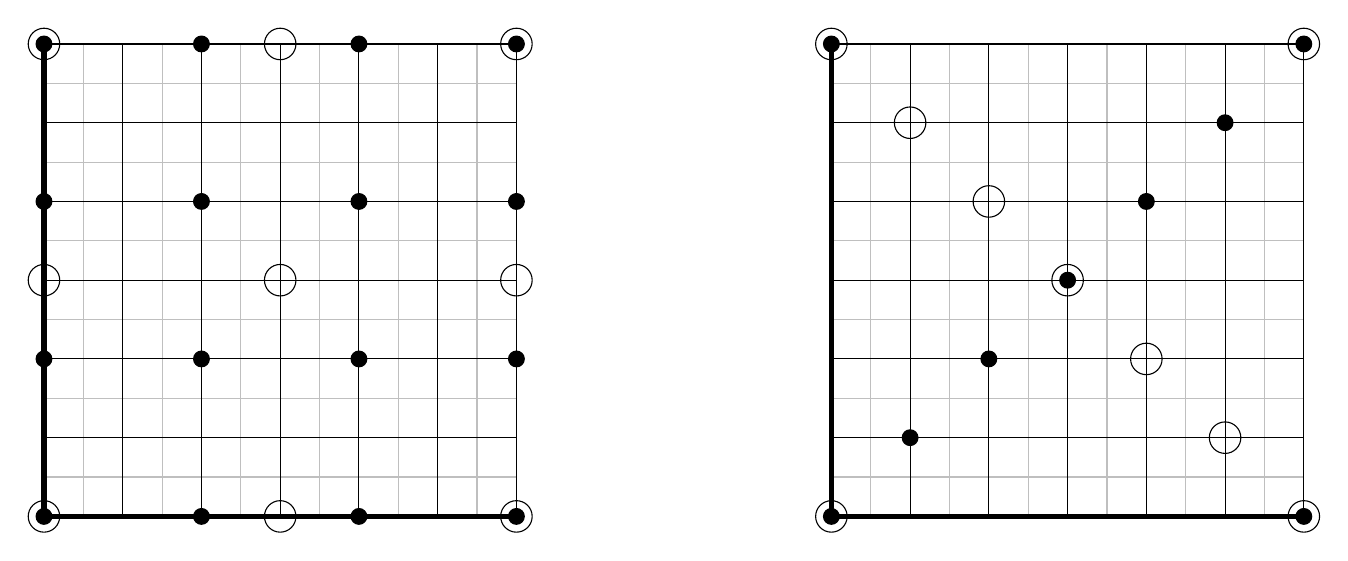
\begin{tikzpicture}[scale=1]

\begin{scope}


\foreach \a in {0,0.5,...,6}{
	\draw[black!25!white] (\a, 0)--(\a,6*1.0);
}

\foreach \a in {0,0.5,...,6}{
	\draw[black!25!white] (0,\a*1.0)--(6,\a*1.0);
}

\foreach \a in {0,...,6}{
	\draw (\a, 0)--(\a,6*1.0);
}

\foreach \a in {0,...,6}{
	\draw (0,\a*1.0)--(6,\a*1.0);
}

\draw[line width=2] (0,0)--(0,6*1.0);
\draw[line width=2] (0,0)--(6,0);

\draw[fill=black] (0,0*1.0) circle (0.1);
\draw[fill=black] (2,0*1.0) circle (0.1);
\draw[fill=black] (4,0*1.0) circle (0.1);
\draw[fill=black] (6,0*1.0) circle (0.1);

\draw[fill=black] (0,2*1.0) circle (0.1);
\draw[fill=black] (2,2*1.0) circle (0.1);
\draw[fill=black] (4,2*1.0) circle (0.1);
\draw[fill=black] (6,2*1.0) circle (0.1);

\draw[fill=black] (0,4*1.0) circle (0.1);
\draw[fill=black] (2,4*1.0) circle (0.1);
\draw[fill=black] (4,4*1.0) circle (0.1);
\draw[fill=black] (6,4*1.0) circle (0.1);

\draw[fill=black] (0,6*1.0) circle (0.1);
\draw[fill=black] (2,6*1.0) circle (0.1);
\draw[fill=black] (4,6*1.0) circle (0.1);
\draw[fill=black] (6,6*1.0) circle (0.1);


\draw (0,0*1.0) circle (0.2);
\draw (3,0*1.0) circle (0.2);
\draw (6,0*1.0) circle (0.2);

\draw (0,3*1.0) circle (0.2);
\draw (3,3*1.0) circle (0.2);
\draw (6,3*1.0) circle (0.2);

\draw (0,6*1.0) circle (0.2);
\draw (3,6*1.0) circle (0.2);
\draw (6,6*1.0) circle (0.2);

\end{scope}

\begin{scope}[xshift=10cm]


\foreach \a in {0,0.5,...,6}{
	\draw[black!25!white] (\a, 0)--(\a,6*1.0);
}

\foreach \a in {0,0.5,...,6}{
	\draw[black!25!white] (0,\a*1.0)--(6,\a*1.0);
}

\foreach \a in {0,...,6}{
	\draw (\a, 0)--(\a,6*1.0);
}

\foreach \a in {0,...,6}{
	\draw (0,\a*1.0)--(6,\a*1.0);
}

\draw[line width=2] (0,0)--(0,6*1.0);
\draw[line width=2] (0,0)--(6,0);

\draw[fill=black] (0,0*1.0) circle (0.1);
\draw[fill=black] (1,1*1.0) circle (0.1);
\draw[fill=black] (2,2*1.0) circle (0.1);
\draw[fill=black] (3,3*1.0) circle (0.1);
\draw[fill=black] (4,4*1.0) circle (0.1);
\draw[fill=black] (5,5*1.0) circle (0.1);
\draw[fill=black] (6,6*1.0) circle (0.1);

\draw[fill=black] (6,0*1.0) circle (0.1);
\draw[fill=black] (0,6*1.0) circle (0.1);

\draw (0,0) circle (0.2);
\draw (6,6) circle (0.2);

\draw (0,6*1.0) circle (0.2);
\draw (1,5*1.0) circle (0.2);
\draw (2,4*1.0) circle (0.2);
\draw (3,3*1.0) circle (0.2);
\draw (4,2*1.0) circle (0.2);
\draw (5,1*1.0) circle (0.2);
\draw (6,0*1.0) circle (0.2);

\end{scope}

\end{tikzpicture} \\ \\
A quick look at this diagram shows that the LCM of $2$ and $3$ is $6$.  But this is also the LCM of $1 + \sqrt{-5}$ and $1-\sqrt{-5}$ is $6$.  This tells us our bookkeeping methods need to get supplemented quite a bit. \\ \\
How and why do continued fractions occur?  Did we get all the mileage we can out of such a construction?  If we complain these objects are useless, maybe it's possible to design a better one.  \\ \\ 
Let's try an example over $\mathbb{Z}$.  Hoping, maybe it can be extended to $\mathbb{Z}[\sqrt{-5}]$.  We can show that since $\pi < 5 $ there is no GCD in this domain.  Euclidean geometry doesn't just finish\dots what's left of that?   \\ \\
\textbf{Thm} Let $\theta$ and $Q> 1$ be real.\footnote{What's coming is yet another very thorough check of the construction of $\mathbb{R}$.  It's supposed to look and feel like a ruler, more or less.  Was the thing you measured even flat?? Did you have all the numbers in between $2$ and $3$ ?} There is an integer such that $0 < q < Q$ and $||q \theta|| < Q^{-1}$. \\ \\
\textit{Proof \#1} \dots \\ \\ 
\textit{Proof \#2} \dots \\ 

\end{document}